Convolution neural network (CNN)\textsuperscript{\cite{cnn}} คือโมเดลปัญญาประดิษฐ์ประเภทหนึ่งที่นิยมนำมาใช้กับงานที่เกี่ยวกับการจำแนกวัตถุในภาพ เช่น แมว หมา มนุษย์ รถ เป็นต้น
กระบวนการที่ CNN จะสามารถจำแนกภาพออกมาได้ว่าเป็นหมวดหมู่อะไรนั้น จะต้องผ่านชั้นกระบวนการต่างๆ เช่น ชั้นตัวกรอง (filter) หรือเคอร์เนล (kernel) , ชั้น pooling layer 
เพื่อสกัดคุณลักษณะ (extract feature) ส่วนชั้น fully connected layer  จะรวบรวมคุณลักษณะทั้งหมด และใช้ softmax หรือ logistic function  สำหรับใช้ในการจำแนกว่าเป็นวัตถุหมวดหมู่อะไร ดังรูปที่ \ref{fig:CNN architecture}

\begin{figure}[!ht]
	\centering
	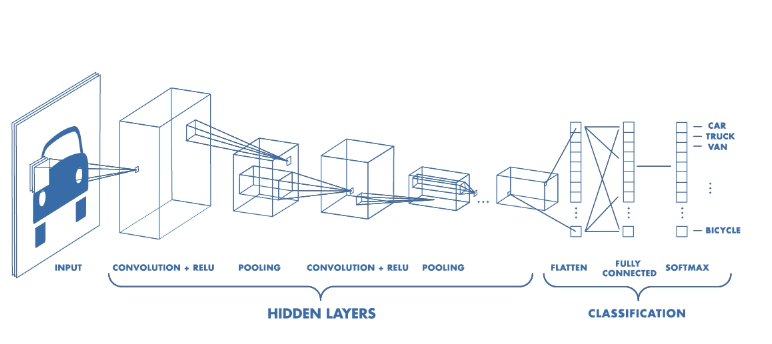
\includegraphics[width=0.8\textwidth]{chapter2/images/CNN.png}
		\caption[ตัวอย่างโครงสร้างของ CNN ที่ใช้ในการจำแนกหมวดหมู่ของวัตถุ]{ตัวอย่างโครงสร้างของ CNN ที่ใช้ในการจำแนกหมวดหมู่ของวัตถุ\textsuperscript{\cite{cnn}}}
    	\label{fig:CNN architecture}
\end{figure}

\subsubsection{ตัวกรอง/เคอร์เนล}
ตัวกรองหรือเคอร์เนล คือชั้นที่ใช้ในการสกัดคุณลักษณะของรูปภาพออกมาด้วยสี่เหลี่ยมเล็กๆขนาด NxN โดยที่ N$\in$[1, 2, 3, ...] ดังรูปที่ \ref{fig:kernel_3x3} 
และสมมติให้ภาพที่ใช้ในการประมวลผลเป็นดังรูปที่ \ref{fig:input_ex}
\begin{figure}[!ht]
	\centering
	\begin{subfigure}[b]{0.5\textwidth}
        \centering
        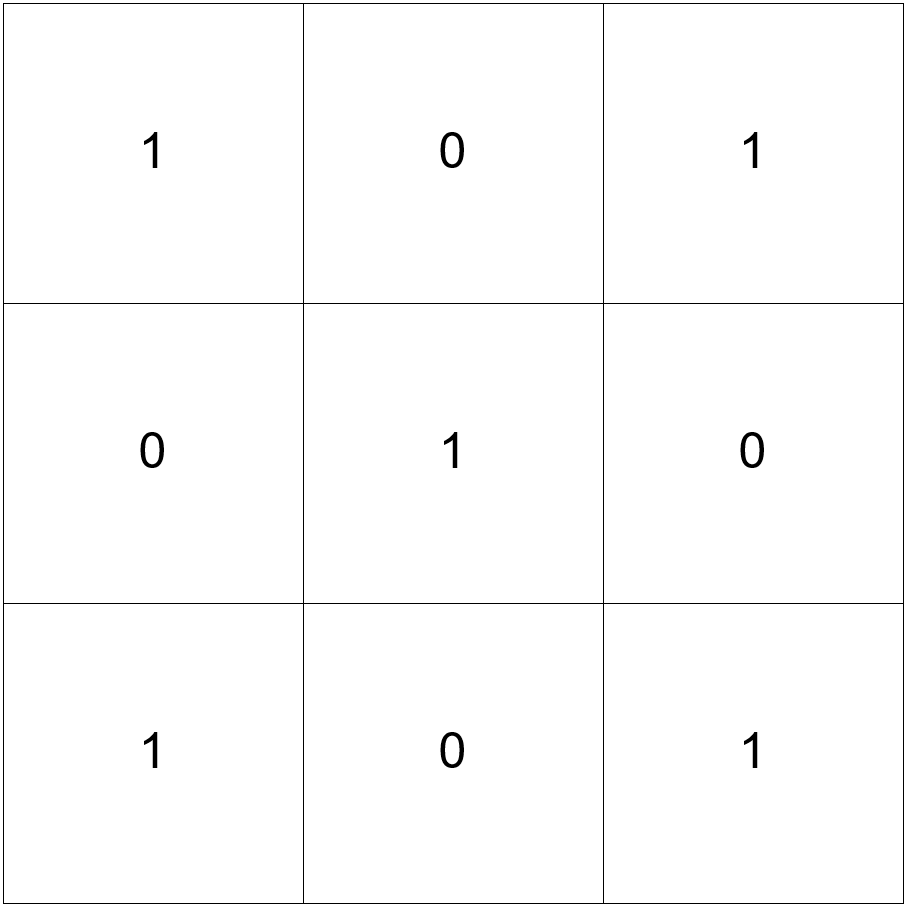
\includegraphics[width=0.4\textwidth]{chapter2/images/kernel_ex.png}
		\caption{ตัวอย่างเคอร์เนลขนาด 3x3}
		\label{fig:kernel_3x3}
    \end{subfigure}
    \begin{subfigure}[b]{0.5\textwidth}
        \centering
		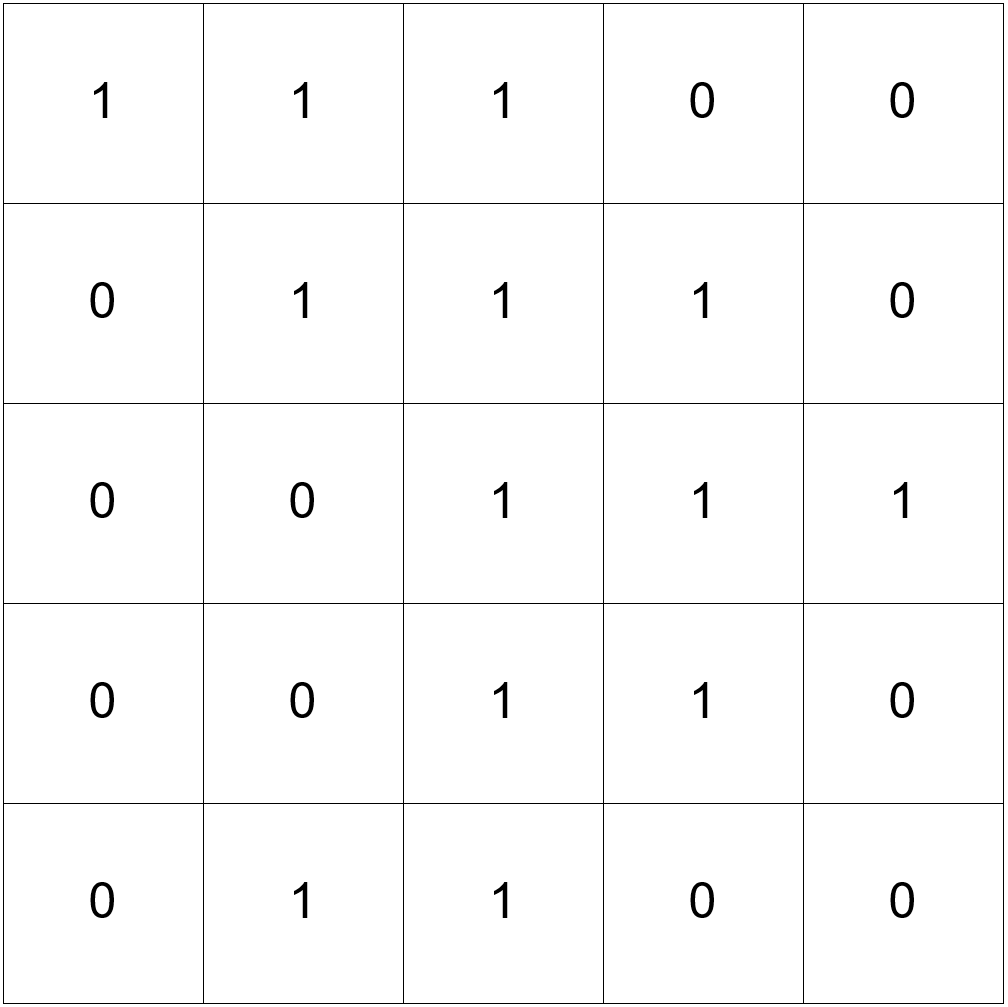
\includegraphics[width=0.5\textwidth]{chapter2/images/input_ex.png}
		\caption{ตัวอย่างภาพที่ใช้ในการประมวลผล}
        \label{fig:input_ex}
	\end{subfigure}
	\caption{ตัวอย่างเคอร์เนล และภาพที่ใช้ในการประมวลผล}
	\label{fig:kernel_input_ex}
\end{figure}
\clearpage
เมื่อนำเคอร์เนล (รูปที่ \ref{fig:kernel_3x3}) ไปทาบกับภาพ (รูปที่ \ref{fig:input_ex}) แล้วคูณค่าในเคอร์เนลกับพิกเซล (pixel) ที่ทาบจะได้คุณลักษณะของช่องนั้นจากนั้นเลื่อนต่อไปจนครบทั้งรูป 
ซึ่งระยะในการเลื่อนนั้นขึ้นอยู่กับผู้สร้างว่าต้องการจะให้เลื่อนครั้งละกี่ช่อง แต่ระยะการเลื่อนที่มากขึ้นจะทำให้ความสัมพันธ์ของคุณลักษณะที่ได้ออกมาน้อยลง โดยการวางเคอร์เนลเทียบบนภาพนั้นจะวางไม่ให้เกินกรอบรูป 
แต่ถ้าต้องการทาบกับทุกพิกเซลในภาพสามารถทำได้ด้วยการให้พื้นที่ที่เกินขอบภาพไปเท่ากับ 0 เทคนิคนี้เรียกว่า padding และคุณลักษณะที่ได้ออกมาทั้งหมดจะเรียกว่าผังคุณลักษณะ (features map) ตามรูปที่ \ref{fig:example feature map}

\begin{figure}[!ht]
	\centering
	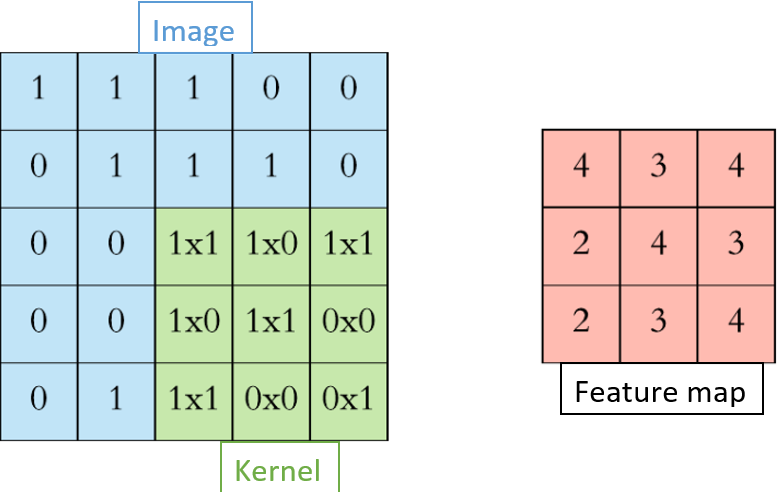
\includegraphics[width=0.5\textwidth]{chapter2/images/feature_map.png}
		\caption[ตัวอย่างการหาผังคุณลักษณะ]{ตัวอย่างการหาผังคุณลักษณะ\textsuperscript{\cite{cnn}}}
    	\label{fig:example feature map}
\end{figure}

\subsubsection{Pooling}
Pooling คือชั้นที่สามารถลดขนาดของภาพลงเพื่อลดข้อมูลที่ไม่จำเป็นลง ซึ่งมีหลายประเภทแต่นิยมใช้มีสองประเภทได้แก่ max pooling และ average pooling
โดยที่ max pooling จะใช้ในการหาค่าที่มากที่สุดในเคอร์เนลที่ทาบอยู่ดังรูปที่ \ref{fig:example max pooling} ในขณะที่ average pooling 
จะหาค่าเฉลี่ยของภายในเคอร์เนลออกมาดังรูปที่ \ref{fig:example average pooling}
\begin{figure}[!ht]
	\centering
	\begin{subfigure}[b]{1.0\textwidth}
		\centering
		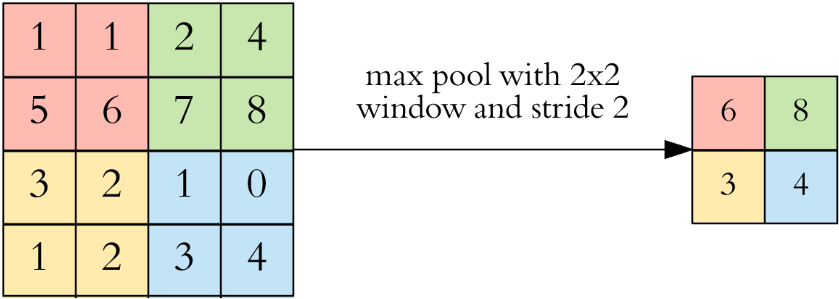
\includegraphics[width=0.5\textwidth]{chapter2/images/max_pooling.png}
		\caption{ตัวอย่างการทำ max pooling\textsuperscript{\cite{cnn}}}
		\label{fig:example max pooling}
    \end{subfigure}
    \begin{subfigure}[b]{1.0\textwidth}
        \centering
		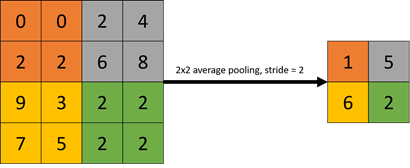
\includegraphics[width=0.5\textwidth]{chapter2/images/average_pooling.png}
		\caption{ตัวอย่างการทำ average pooling\textsuperscript{\cite{average_pooling}}}
		\label{fig:example average pooling}
	\end{subfigure}
	\caption{ตัวอย่างการใช้ max pooling และ average pooling กับภาพ}
	\label{fig:pooling_ex}
\end{figure}
\clearpage

\subsubsection{Activation function\textsuperscript{\cite{activation}}}
ในแต่ละชั้นของ CNN นั้นจะมี activation function เป็นสิ่งที่กำหนดว่าผลลัพธ์ของชั้นนั้นว่าจะอยู่ในช่วงไหน 
เช่น -1 ถึง 1, 0 ถึง 1 ขึ้นอยู่กับฟังก์ชันที่ใช้ ซึ่งจะแบ่งออกเป็นสองแบบคือ แบบเป็นเส้นตรงและแบบไม่เป็นเส้นตรง

แบบเป็นเส้นตรงจะมีสมการของฟังก์ชันดังนี้ $ f(x) = x $ โดยที่ $x$ คือข้อมูลป้อนเข้าของฟังก์ชัน ทำให้ผลลัพธ์ที่ได้จากฟังก์ชันนี้มีค่าอยู่ในช่วง -inf ถึง inf
ส่วนในแบบไม่เป็นเส้นตรงจะมีหลายฟังก์ชัน แต่ฟังก์ชันที่เป็นที่นิยมใช้คือ Rectified Linear Unit หรือ ReLU, Leaky ReLU และ Parametric ReLU โดยทั้งสามฟังก์ชันมีสมการดังนี้\\
\textbf{ReLU}\\
$ f(x) =
\begin{cases}
	0 & \text{if } x < 0,\\
	x & \text{otherwise}
\end{cases}
$\\
\textbf{Leaky ReLU}\\
$ f(x) =
\begin{cases}
	0.01x & \text{if } x < 0,\\
	x & \text{otherwise}
\end{cases}
$\\
\textbf{Parametric ReLU} โดยที่ $\alpha\in\mathbb{R^+}$\\
$ f(x) =
\begin{cases}
	\alpha x & \text{if } x < 0,\\
	x & \text{otherwise}
\end{cases}
$
\subsubsection{Fully connected layer}
เป็นชั้นที่จะรวมคุณลักษณะทั้งหมดของชั้นก่อนหน้าให้เป็นเวกเตอร์ (vector) ก่อนที่จะนำไปคำนวณด้วย activation function เพื่อหาคำตอบสำหรับการจำแนกหมวดหมู่ของภาพ
ซึ่งฟังก์ชันที่นิยมใช้จะมีสองฟังก์ชัน คือ softmax และ sigmoid (logistic) โดยทั้งสองมีความแตกต่างกันดังตารางที่ \ref{tab:softmax_vs_sigmoid}
\begin{table}[!ht]
	\centering
	\begin{tabular}{|c|c|c|}
		\hline
		{} & Softmax & Sigmoid\\
		\hline\hline
		1 & \begin{tabular}{@{}c@{}}สมการคือ $f(x_i) = \frac{exp(x_i)}{\sum_{j=0}^k exp(x_j)}$ \\โดยที่ k คือจำนวนข้อมูล และ i$\in${0, 1, 2, ..., k}\end{tabular} & $f(x_i) = \frac{1}{1+exp(-x_i)}$ โดยที่ i$\in${0, 1, 2, ..., k}\\
		\hline
		2 & ผลรวมของความน่าจะเป็นจะเท่ากับ 1 เสมอ & ผลรวมของความน่าจะเป็นไม่จำเป็นต้องเท่ากับ 1\\
		\hline
		3 & มักใช้ในการจำแนกหมวดหมู่มากกว่าสองหมวดหมู่ขึ้นไป & มักใช้ในการจำแนกหมวดหมู่เพียงสองหมวดหมู่\\
		\hline
	\end{tabular}
	\caption{ตารางแสดงการเปรียบเทียบระหว่าง softmax function และ sigmoid function}
	\label{tab:softmax_vs_sigmoid}
\end{table}
\clearpage

\subsubsection{Intersection over union (IoU)}
\begin{figure}[!ht]
	\centering
	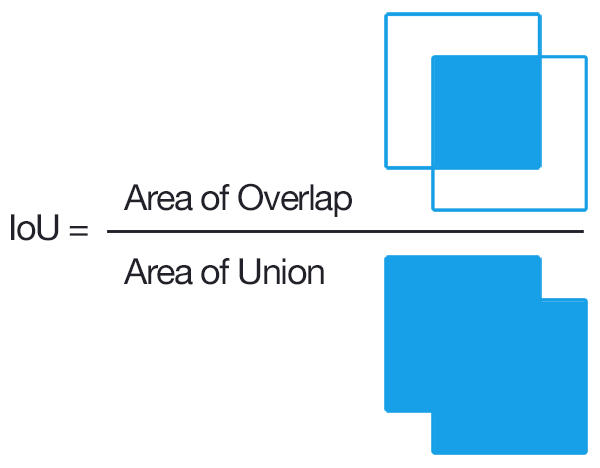
\includegraphics[scale=0.3]{chapter2/images/iou_equation.png}
		\caption[ภาพแสดงการหา IoU ด้วยการใช้กรอบสี่เหลี่ยมซึ่งเป็นคำตอบจริงและกรอบสี่เหลี่ยมที่ได้จากการทำนาย]{ภาพแสดงการหา IoU ด้วยการใช้คำตอบจริงของการทำนายและกรอบสี่เหลี่ยมที่ได้จากการทำนาย\textsuperscript{\cite{iou_pic}}}
    	\label{fig:iou_equation}
\end{figure}
เป็นวิธีในการทดสอบประสิทธิภาพของการตรวจจับวัตถุ โดยค่า IoU นั้นสามารถหาได้จากการนำกรอบสี่เหลี่ยมจริงของวัตถุและกรอบสี่เหลี่ยมที่ได้จากการทำนาย
มาหาอัตราส่วนระหว่างพื้นที่ที่กรอบสี่เหลี่ยมทั้งสองทับซ้อนกัน และหารด้วยพื้นที่ทั้งหมดของกรอบสี่เหลี่ยมทั้งสองรวมกัน ซึ่งสามารถเขียนในรูปสมการได้ดังนี้
\begin{equation}
IoU(P,G) = \frac{\left| P \cap G \right|}{\left| P \cup  G \right|}					
\end{equation}
โดยที่
\begin{conditions}
IoU			&  ค่าที่ใช้สำหรับวัดผลความใกล้เคียงระหว่างสองกรอบสี่เหลี่ยม    \\
P			&  พื้นที่ของกรอบสี่เหลี่ยมที่ทำนายได้	\\
G			&  พื้นที่ของกรอบสี่เหลี่ยมจริงของรูปภาพ					\\
\end{conditions}

\subsubsection{Area under the curve (AUC) - Receiver Operating Characteristics Curve (ROC)}
AUC - ROC\textsuperscript{\cite{auc_roc}} เป็นวิธีในการทดสอบประสิทธิภาพการแยกแยะของโมเดลปัญญาประดิษฐ์ โดยที่ ROC คือเส้นโค้งของความน่าจะเป็น และ AUC คือค่าที่บ่งบอกถึงความสามารถในการแยกแยะ ค่า AUC จะอยู่ในช่วง 0 - 1 ถ้าค่า AUC ใกล้เคียง 1 มากเท่าไหรก็จะหมายถึงความสามารถในการแยกแยะของโมเดลปัญญาประดิษฐ์สูงตามไปด้วย

\begin{figure}[!ht]
	\centering
	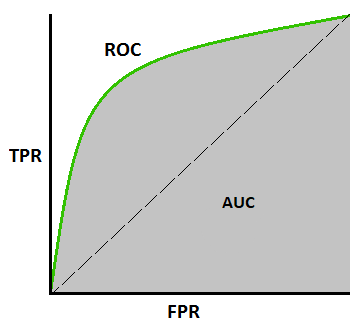
\includegraphics[scale=0.3]{chapter2/images/auc_roc.png}
		\caption[AUC - ROC Curve]{AUC - ROC Curve\textsuperscript{\cite{auc_roc}}}
    	\label{fig:auc_roc}
\end{figure} 

จากรูปที่ \ref{fig:auc_roc} เส้นโค้ง ROC สามารถหาได้ด้วยการนำค่า True positive rate (TPR) และ False positive rate (FPR) มาสร้างเป็นกราฟ โดยค่า TPR จะอยู่ในแกน y และค่า FPR จะอยู่ในแกน x ซึ่งสามารถหาค่าของ TPR และ FPR ได้ดังนี้

\begin{equation}
TPR = \frac{TP}{TP + FN}
\end{equation}
โดยที่
\begin{conditions}
TP		&		จำนวนของข้อมูลที่มีผลลัพธ์เป็นจริงและผลจากโมเดลปัญญาประดิษฐ์เป็นจริง		\\
FN		&		จำนวนของข้อมูลที่มีผลลัพธ์เป็นจริงและผลจากโมเดลปัญญาประดิษฐ์เป็นเท็จ
\end{conditions}

\begin{equation}
FPR = \frac{FP}{FP + FN}
\end{equation}
โดยที่
\begin{conditions}
FP		&		จำนวนของข้อมูลที่มีผลลัพธ์เป็นเท็จและผลจากโมเดลปัญญาประดิษฐ์เป็นจริง		\\
FN		&		จำนวนของข้อมูลที่มีผลลัพธ์เป็นจริงและผลจากโมเดลปัญญาประดิษฐ์เป็นเท็จ
\end{conditions}

\subsubsection{Non Maximum Suppression (NMS)}
Non Maximum Suppression\textsuperscript{\cite{nms}} คือ อัลกอริทึม (algorithm) ที่นิยมใช้เข้ามาช่วยจัดการปัญหากรอบสี่เหลี่ยมที่ซ้อนทับกันซึ่งเกิดจากการทำนายวัตถุเดียวกันในพื้นที่บริเวณใกล้ๆ เพื่อให้ได้กรอบสี่เหลี่ยมที่บ่งบอกถึงตำแหน่งของวัตถุนั้นเพียงกรอบเดียว จึงมีการนำเอาอัลกอริทึ่ม nms เข้ามาช่วยแก้ไขปัญหา 
\begin{figure}[!ht]
	\centering
	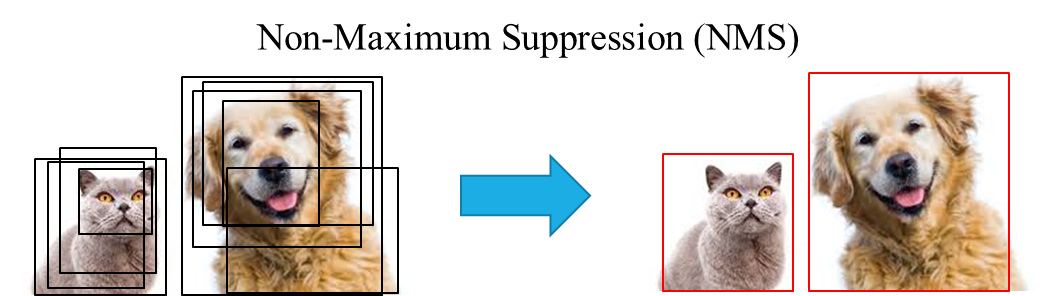
\includegraphics[scale=0.3]{chapter2/images/NMS.png}
		\caption[ตัวอย่างการทำงานของ NMS]{ตัวอย่างการทำงานของ NMS\textsuperscript{\cite{nms_pic}}}
    	\label{fig:NMS}
\end{figure}

\subsubsection{Optimization algorithm}
ในขั้นตอนการสร้างโมเดลปัญญาประดิษฐ์นั้นสิ่งที่สำคัญคือ การลดความผิดพลาด (error) หรือค่าคอสท์ (cost) นั่นทำให้ต้องมีเครื่องมือสำหรับปรับพารามิเตอร์ของโมเดลเพื่อให้มีความผิดพลาดน้อยที่สุด
นั่นทำให้มีการคิดค้น optimization algorithm ต่างๆขึ้นมา ตัวอย่างเช่น gradient descent (GD), Momentum, RMS Prop และ Adam เป็นต้น
ซึ่งเมทริกซ์ weight มักจะสุ่มค่าในตอนต้น แล้วใช้ optimization algorithm ในการลดค่าคอสท์ที่ได้จาก cost funtion พร้อมทั้งหาเมทริกซ์ weight และค่าอคติ (bias) ที่ดีที่สุด
โดยจากตัวอย่างที่ยกไปก่อนหน้านี้แต่ละอัลกอริทึมนั้นมีรายละเอียดดังนี้
\begin{enumerate}
	\item Gradient descent (GD) เป็นอัลกอริทึมที่จะทำการปรับเมทริกซ์ weight และค่าอคติของทุกข้อมูลที่ใช้ในการสร้างโมเดล โดยจะมีสมการดังนี้
	\begin{equation}
		W = W - \alpha \frac{\partial J(W)}{\partial W}
	\end{equation}
	\begin{equation}
		b = b - \alpha \frac{\partial J(b)}{\partial b}
	\end{equation}
	โดยที่
	\begin{conditions}
		W & เมทริกซ์ weight\\
		\alpha & อัตราการเรียนรู้ (learning rate)\\
		J & cost function\\
		b & ค่าอคติ
	\end{conditions}
	สมการแรกนั้นคือสมการการปรับเมทริกซ์ weight ในขณะที่สมการที่สองคือสมการปรับค่าอคติ ซึ่งทั้งสองสมการนั้นจะมีอัตราการเรียนรู้เป็นตัวกำหนดอัตราการเปลี่ยนแปลง จากรูปที่ \ref{fig:gd_explain} จุดสีแดงหมายถึงกรณีที่ weight มีค่าน้อยกว่าค่าที่เหมาะสมในจุดสีม่วง จากรูปจะเห็นว่าความชัน ณ จุดสีแดงเมื่อเทียบกับจุดสีม่วง มีค่าเป็นลบทำให้เมื่อนำไปใส่ในสมการแล้วจะทำให้มีการปรับ weight ให้เพิ่มขึ้น ในทางตรงกันข้ามที่จุดสีน้ำเงินเมื่อเทียบกับจุดสีม่วงจะมีความชันเป็นบวกทำให้มีการปรับ weight ให้น้อยลง  ซึ่งการปรับแต่ละครั้งจะมีระยะก้าวกว้างขนาดไหนจะขึ้นอยู่กับอัตราการเรียนรู้ดังตัวอย่างในรูปที่ \ref{fig:learning_rate}
	\begin{figure}
		\begin{subfigure}[!ht]{0.5\textwidth}
			\centering
			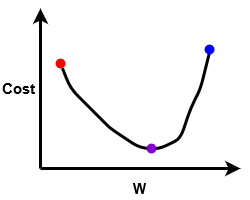
\includegraphics[width=0.5\textwidth]{chapter2/images/gd_explain.png}
				\caption{กราฟสำหรับอธิบายการทำงานของ gradient descent}
				\label{fig:gd_explain}
		\end{subfigure}
		\begin{subfigure}[!ht]{0.5\textwidth}
			\centering
			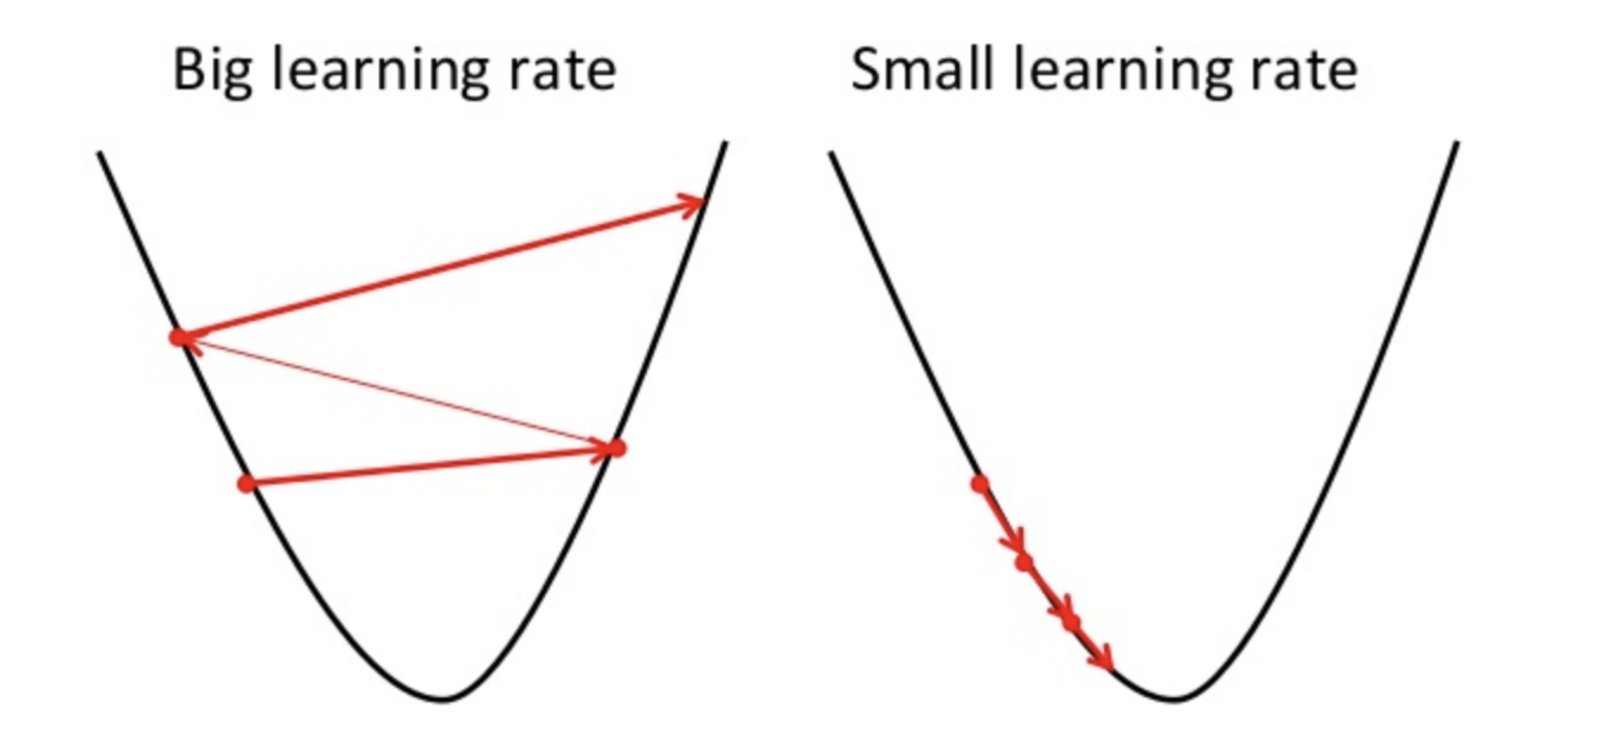
\includegraphics[width=0.85\textwidth]{chapter2/images/learning_rate.png}
				\caption{ตัวอย่างผลลัพธ์ของการปรับค่าอัตราการเรียนรู้ที่ต่างกัน}
				\label{fig:learning_rate}
		\end{subfigure}
		\caption{รูปสำหรับอธิบายการทำงานของ gradient descent}
		\label{fig:gd_figure}
	\end{figure}
	
	ข้อเสียของ gradient descent คือจะทำการปรับค่าพารามิเตอร์หลังจากทำการคำนวณจนครบทุกข้อมูลในชุดข้อมูลที่ใช้ในการสร้างแล้วเท่านั้น ทำให้เกิดปัญหาหน่วยความจำไม่เพียงพอเมื่อใช้กับชุดข้อมูลที่มีขนาดที่ใหญ่มาก
	จึงทำให้เกิดเทคนิคที่เรียกว่า stochastic gradient descent (SGD) กล่าวคือถ้าหาก gradient descent ทำการคำนวณจนครบทุกข้อมูลจึงจะมีการปรับพารามิเตอร์ ส่วน stochastic gradient descent จะคำนวณเพียงข้อมูลหนึ่งตัวหรือเป็นชุดของข้อมูล (subset) ซึ่งหากใช้เป็นชุดของข้อมูลจะเรียกว่า minibatch stochastic gradient descent การทำแบบนี้จะทำให้ลดการใช้หน่วยความจำลง 
	และทำให้การสร้างโมเดลนั้นทำได้เร็วขึ้นกว่าการใช้ gradient descent
	\item Momentum หรือ gradient descent with momentum มีการทำงานเหมือนกับ gradient descent แต่จะมีการเร่งความเร็วในการปรับลดค่าจาก cost function โดยใช้สิ่งที่เรียกว่าค่าเฉลี่ยเคลื่อนที่
	(moving average) เพื่อลบข้อมูลรบกวน โดยสามารถหาได้จากสมการดังนี้
	\begin{equation}
		V_{dW} = \beta V_{dW} + (1 - \beta)dW
	\end{equation}
	\begin{equation}
		V_{db} = \beta V_{db} + (1 - \beta)db
	\end{equation}
	โดยที่
	\begin{conditions}
		V_{dW}	&	moving average ของอนุพันธ์ของเมทริกซ์ weight\\
		\beta	&	พารามิเตอร์ของ moving average (ค่าคงที่ momentum)\\
		dW		&	อนุพันธ์ของเมทริกซ์ weight\\
		V_{db}	&	moving average ของอนุพันธ์ของค่าอคติ\\
		db		&	อนุพันธ์ของค่าอคติ
	\end{conditions}
	ในการสร้างโมเดลปัญญาประดิษฐ์นั้นมีเป้าหมายถึงคือการหา cost function ที่เหมาะสมเพื่อให้ได้ค่าความผิดพลาดน้อยที่สุด หากดูจากรูปที่ \ref{fig:momentum_explain} 
	gradient descent จะเป็นไปตามเส้นสีแดง ในขณะที่ momentum จะเป็นเส้นสีเขียว และจุดสีม่วงคือจุดที่มีค่าความผิดพลาดน้อยที่สุด จะเห็นว่า gradient descent แกว่งมากในแกน y 
	แต่มีการเคลื่อนที่ในแกน x เพียงเล็กน้อย วิธีแก้คือทำให้การแกว่งในแกน y น้อยลง นั่นทำให้มีการใช้ค่าเฉลี่ยเคลื่อนที่เข้ามาช่วย ทำให้สมการปรับ weight และค่าอคติเปลี่ยนเป็นดังสมการด้านล่าง
	\begin{equation}
		W = W - \alpha V_{dW}
	\end{equation}
	\begin{equation}
		b = b - \alpha V_{db}
	\end{equation}
	\begin{figure}[!ht]
		\centering
		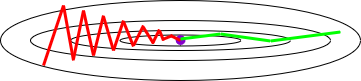
\includegraphics[width=0.7\textwidth]{chapter2/images/momentum_explain.png}
			\caption{เปรียบเทียบการทำงานของ gradient descent กับ Momentum}
			\label{fig:momentum_explain}
	\end{figure} 
	\item RMS Prop หรือ root-mean-square propagation ซึ่งมีความคล้ายคลึงกับ Momentum หากดูจากรูปที่ \ref{fig:momentum_explain} กำหนดให้แกน y เป็นค่าอคติ แกน x คือ weight
	และเส้นสีเขียวเป็นของ RMS Prop ในขณะที่ momentum ใช้ค่าเฉลี่ยเคลื่อนที่ในการลดการแกว่งในแนวแกน y RMS Prop จะใช้ค่าเฉลี่ยกำลังสองมาหารเพื่อลดการแกว่งในแกน y ซึ่งทำให้ต้องมีค่าคงที่ $\epsilon$
	เพื่อไม่ให้เกิดเหตุการณ์หารด้วยศูนย์ ซึ่งสมการปรับ weight และค่าอคติจะเป็นดังนี้
	\begin{equation}
		W = W - \alpha \frac{dW}{\sqrt{S_{dW}} + \epsilon}
	\end{equation}
	\begin{equation}
		b = b - \alpha \frac{db}{\sqrt{S_{db}} + \epsilon}
	\end{equation}
	โดยที่ $S_{dW}$ และ $S_{db}$ สามารถหาได้จากสมการที่ \ref{equa:s_w} และ \ref{equa:s_b} ตามลำดับ
	\begin{equation}
		S_{dW} = \beta S_{dW} + (1 - \beta) dW^2
		\label{equa:s_w}
	\end{equation}\begin{equation}
		S_{db} = \beta S_{db} + (1 - \beta) db^2
		\label{equa:s_b}
	\end{equation}
	\item Adam หรือ Adaptive momentum เป็นอัลกอริทึมที่นำเทคนิคของ momentum และ RMS Prop มารวมกัน ทำให้อัลกอริทึมนี้มีประสิทธิภาพที่สูงและมีความเร็วในการปรับพารามิเตอร์ของโมเดลได้เร็ว 
	ซึ่งได้มีการใช้เทคนิค error correction เพื่อแก้ปัญหา cold start หมายถึงปัญหาที่ในช่วงแรกๆนั้นพารามิเตอร์ของ momentum และ RMS Prop นั้นมีค่าห่างจากค่าจริงมากเกินไปทำให้การปรับพารามิเตอร์เกิดขึ้นช้าเกินไป
	โดยสมการ error correction ของทั้ง momentum และ RMS Prop คือ
	\begin{equation}
		V^{correction}_{dW} = \frac{V_{dW}}{1 - \beta_1}
	\end{equation}
	\begin{equation}
		V^{correction}_{db} = \frac{V_{db}}{1 - \beta_1}
	\end{equation}
	\begin{equation}
		S^{correction}_{dW} = \frac{S_{dW}}{1 - \beta_2}
	\end{equation}
	\begin{equation}
		S^{correction}_{db} = \frac{S_{db}}{1 - \beta_2}
	\end{equation}
	และสมการปรับ weight และค่าอคติของอัลกอริทึมนี้จะเป็นดังสมการด้านล่างนี้ 
	\begin{equation}
		W = W - \alpha \frac{V^{correction}_{dW}}{\sqrt{S^{correction}_{dW}} + \epsilon}
	\end{equation}
	\begin{equation}
		b = b - \alpha \frac{V^{correction}_{db}}{\sqrt{S^{correction}_{db}} + \epsilon}
	\end{equation}
\end{enumerate}